\documentclass{article}
\usepackage{amsmath}
\usepackage[margin=0.75in]{geometry}
\usepackage{graphicx}
\setcounter{MaxMatrixCols}{20}
\begin{document}
\title{Econometrics Assignment 1}
\author{Eric Tu}
\maketitle
\begin{enumerate}
%1
	\item This exercise considers an example of data that do not satisfy all the standard assumptions of simple regression.
In the considered case, assumption A6 that the coefficients α and β are the same for all observations is violated.
The dataset contains survey outcomes of a travel agency that wishes to improve recommendation strategies for its
clients. The dataset contains 26 observations on age and average daily expenditures during holidays.
\\
	%a
	\begin{enumerate}
		\item Use all data to estimate the coefficients a and b in a simple regression model, where expenditures is the
dependent variable and age is the explanatory factor. Also compute the standard error and the t-value of b. \\

		\begin{center}
		Using the attached R code, the simple regression model $y = a + bx$ on the dataset results in: \\
		$\begin{matrix}
		a: 141.7 && Std Error: 29.3112 && tvalue: 4.834 \\
		b: -1.01 && Std Error: 0.2894 && tvalue: -3.498  \\
		\end{matrix}$
		
		
		\end{center}

	%b
		\item Make the scatter diagram of expenditures against age and add the regression line y = a + bx of part (a) in
this diagram. What conclusion do you draw from this diagram? \\
		\begin{center}
			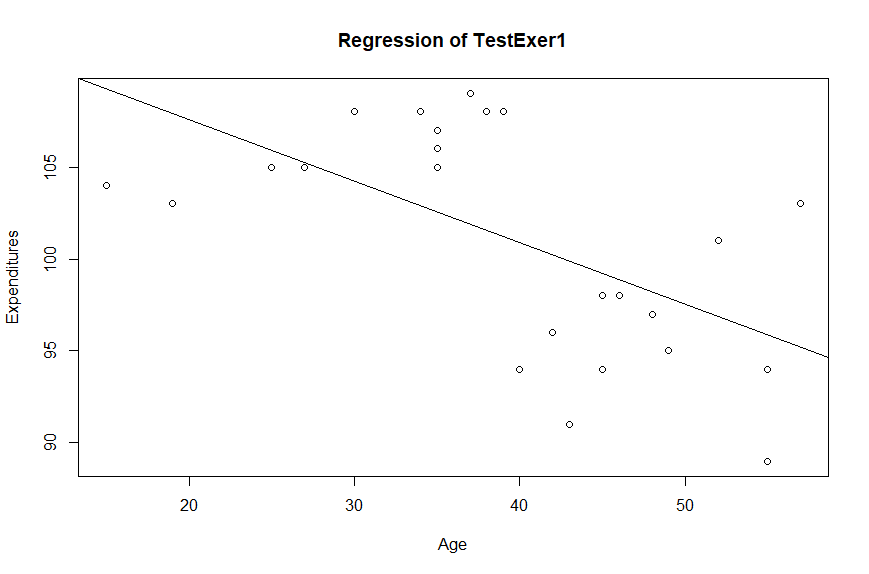
\includegraphics[scale=0.5]{Rplot.png} \\
			The regression line draws a reasonable fit along the points, showing an inverse relationship between age and expenditures.
		\end{center}


	%c
		\item It seems there are two sets of observations in the scatter diagram, one for clients aged 40 or higher and
another for clients aged below 40. Divide the sample into these two clusters, and for each cluster estimate the
coefficients a and b and determine the standard error and t-value of b. \\
		\begin{center}
			For the Age $< 40$ Group:
			$\begin{matrix}
			a: 100.2 && Std Error: 1.42 && tvalue: 70.79 \\
			b: 0.20 && Std Error: 0.04 && tvalue: 4.46  \\
			\end{matrix}$
			\\
			For the Age $\geq 40$ Group:
			$\begin{matrix}
			a: 88.9 && Std Error: 9.45 && tvalue: 9.40 \\
			b: 0.15 && Std Error: 0.20 && tvalue: 0.74  \\
			\end{matrix}$
			\\
		\end{center}

	%d
		\item Discuss and explain the main differences between the outcomes in parts (a) and (c). Describe in words what
you have learned from these results. \\

		\begin{center}
			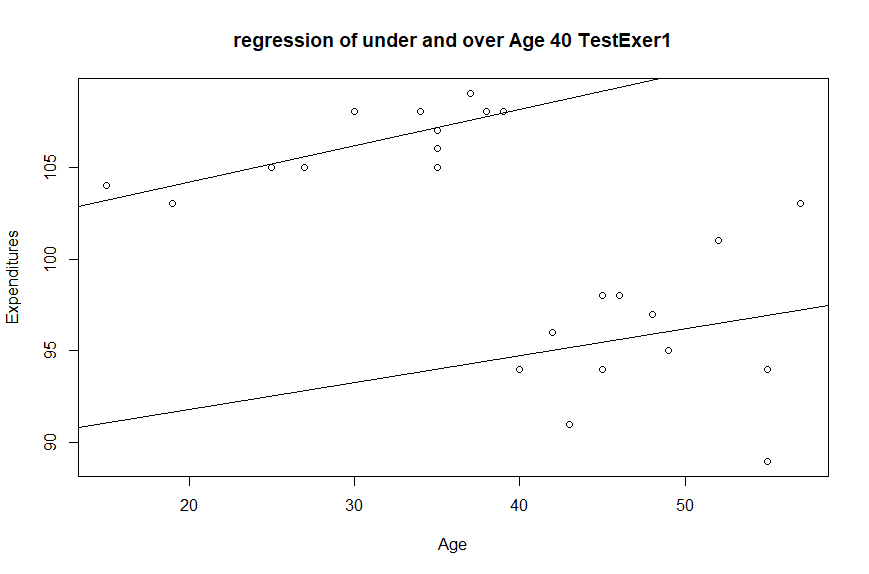
\includegraphics[scale=0.5]{splitRplot.png}		\\	
			The regression lines in c show an upward trend instead of the downware trend seen in part a. This shows cleaning the data is an important task, and that regression of subsets of data may be more meaningful than a regression over the entire set. \\
		\end{center}
	\end{enumerate}		
		
R code...\\
library("xlsx") \\
data <- read.xlsx("TrainExer13.xls", 1) \\

\# a - Use all data to estimate coefficients a and b in simple regression line \\
fit <- lm(Expenditures ~ Age, data=data) \\
summary(fit)\\

\#b Plot best fit line\\
plot(Expenditures ~ Age, data=data, main='regression of TestExer1')\\
abline(fit)\\

\#c Split data into two sets of observations\\
u40data <- data[data['Age']<40,]\\
a40data <- data[data['Age']>=40,]\\

u40fit <- lm(Expenditures ~ Age, data=u40data)\\
a40fit <- lm(Expenditures ~ Age, data=a40data)\\
summary(u40fit)\\
summary(a40fit)\\

\#Discuss main differences between parts a and c
plot(Expenditures ~ Age, data=data, main='regression of under and over Age 40 TestExer1')\\
abline(u40fit)\\
abline(a40fit)\\


\end{enumerate}

\end{document}